\documentclass[12pt]{article}

\pdfoutput=1
\usepackage[letterpaper, margin=2cm]{geometry}
\usepackage{amsmath, amssymb}
\usepackage{amsthm}
\usepackage{mathtools}
\usepackage{graphicx}
\usepackage{fancyhdr}
\usepackage{cancel}
\usepackage{adjustbox}
\usepackage{multicol}
\usepackage{pdflscape}
\usepackage{pgffor}
\usepackage{tikz}

\usepackage{listings}
\lstset{
    basicstyle=\ttfamily,
    commentstyle=\ttfamily\lst@column@fullflexible,
    showstringspaces=false,
    numbers=left,
    frame=trbl,
    breaklines=true,
}

\usepackage{hyperref}
\hypersetup{
    colorlinks=true,
    linkcolor=blue,
    citecolor=magenta,
    filecolor=magenta,
    urlcolor=blue,
    pdftitle={},
    pdfpagemode=FullScreen,
}


% \documentclass[sigconf, 11pt]{acmart}
% \settopmatter{printacmref=false} % Removes citation information below abstract
% \settopmatter{printfolios=true}
% \renewcommand\footnotetextcopyrightpermission[1]{} % removes footnote with conference information in first column
% \pagestyle{plain} % removes running headers

\usepackage[utf8]{inputenc}
\usepackage[T1]{fontenc}

% %%%%%%%%%%%%%%%%%%%%%%%%%%%%%%%%%%%%%%%%%%%%%%%%%%%%%%%%%%%%%%%
% Sample header file
% This can be replaced if wanted, just included for convenience
%%%%%%%%%%%%%%%%%%%%%%%%%%%%%%%%%%%%%%%%%%%%%%%%%%%%%%%%%%%%%%%

%% Standard packages
\usepackage{amsmath}
\usepackage{microtype}

%% Layout
\usepackage[margin=2.5cm]{geometry}
\usepackage{parskip}

%% Tables
\usepackage{array}
\usepackage{booktabs}
% \usepackage{tabularx}

%% Graphics
\usepackage{graphicx}
\usepackage[dvipsnames]{xcolor}

%% Hyperlinks
\usepackage{url}
\usepackage{hyperref}
\hypersetup{
    colorlinks,
    linkcolor={red!40!black},
    citecolor={blue!50!black},
    urlcolor={blue!80!black}
}

% Theorems and cleveref
% Cleveref must be loaded AFTER amsthm and BEFORE thm definitions.
% See: https://tex.stackexchange.com/questions/19104/cleveref-with-counters-with-same-name
\usepackage{amsthm}
\usepackage{cleveref}

\theoremstyle{definition}
\newtheorem{theorem}{Theorem}
\newtheorem{lemma}[theorem]{Lemma}
\newtheorem{proposition}[theorem]{Proposition}
\newtheorem{definition}[theorem]{Definition}
\newtheorem{example}[theorem]{Example}

%% Tikz
% \usepackage{tikz}
% \usetikzlibrary{positioning, matrix, fit, arrows, shapes}

%% Algorithms
% \usepackage{algorithm, caption}
% \usepackage[noend]{algpseudocode} % (layout for algorithmicx)
% \usepackage{listings}

%% Symbols
\usepackage{amssymb}
% \usepackage{stmaryrd} % Symbols like \llbracket, \rrbracket
% \usepackage{pifont} % Symbols like \ding
% \usepackage{relsize} % Large symbols (\mathlarger)

%%%%%%%%%%%%%%%%%%%%%%%%%%%%%%%%%%%%%%%%%%%%%%%%%%%%%%%%%%%%%%%
% Add custom packages and macros here


\title{Credential Management in Resilient DB (ResCred)\\
    Final Report \\
\large{A Resilient Blockchain-based Credential Management System}\\
}
\author{Avni Bafna, Federico Jimenez, Ethan Ng, Vikram Penumarti, Zhenkai Weng}
\date{\today{}}

\begin{document}

\maketitle

\abstract{
    ResCred is a blockchain-based credential management web application engineered to guarantee quick, tamper-proof, and decentralized verification. ResCred leverages the power of permissioned blockchains to address common challenges in conventional verification processes, including inefficiency, lack of transparency, and susceptibility to fraud or tampering. This web application is integrated with ResilientDB’s blockchain technology to help ensure the authenticity of an individual’s academic, professional, and personal credentials building a trusted and reliable medium of verification.
}

\section{Overview}
By utilizing ResilientDB, a permissioned blockchain, the Resilient DB Credential Management (ResCred) project aims to overcome inefficiencies and opaqueness in current academic/occupational credential verification procedures by developing a decentralized, transparent, and secure credential management system. Conventional verification relies on a small number of authorities to confirm credentials, which are prone to bottlenecks, human mistake, and identity theft.

Through smart contracts, ResCred seeks to democratize and expedite credential issuance and verification. This will allow entities to manage, issue, and revoke credentials while enabling credential holders and verifiers to safely interact with the data. ResCred improves security and efficiency by using decentralized identifiers (DIDs) and cryptographic validation to create a publicly visible, tamper-proof ledger that reduces identity and centralization issues.


\section{Solution}

ResCred (See \autoref{fig:ResCred_description}) is a decentralized web application that utilizes ResilientDB to create a public blockchain to store, verify, and manage credentials, offering:
\begin{enumerate}
    \item Secure Verification \\
        We aim to be able to verify any transaction record in the database via any replica, using asymmetric cryptography to confirm the authenticity of the issuing body.
    \item Efficiency \\
        Automated verification process removes intermediaries from the issuing and verification process, improving reliability and the timeliness of verifying credentials.
    \item Transparency \\
        All transactions on ResCred are logged immutably which prevents tampering of records ensuring trust and accountability.
\end{enumerate}
Each certification will be recorded on ResilientDB as a transaction between an issuing body and a credential holder, allowing anyone to see the issuing and modification history of that record. Only authorized institutions will have the ability to issue, expire, or revoke credentials while remaining publicly accessible and verifiable.

\begin{figure}
    \begin{center}
        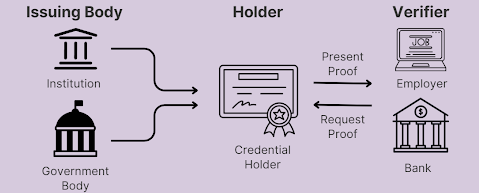
\includegraphics[width=0.95\textwidth]{img/rescred_description.png}
    \end{center}
    \caption{Picture describing ResCred}\label{fig:ResCred_description}
\end{figure}


\section{Technology Stack}
\begin{enumerate}
    \item Web Application: Typescript, CSS, Vue, Vite 
    \item Backend: ResilientDB GraphQL server, Solidity
    \item Database: Powered by ResilientDB Smart Contract Service
\end{enumerate}

\section{Architecture}

\subsection{Frontend}

ResCred frontend is a Vite-compiled static site that has the ability to do HRM/live reload during development thanks to Vite (npm run dev). Due to the Same Origin Policy, we do not want to serve the GraphQL server on a different origin, so we serve both the static frontend and the GraphQL server on a single Nginx reverse proxy. 
We set \verb|/| to redirect to the frontend, and \verb|/graphql| to redirect to the GraphQL API,
which talks to ResContract CLI and the smart contract service behind the firewall.

\subsection{Backend}

Thanks to the power of the Ethereum Virtual Machine, ResCred’s real backend is technically made up of smart contracts, accessed via several layers of indirection: GraphQL API, ResContract CLI, and smart contract service.

Before the app goes online, a version of the \verb|Registry| contract needs to be deployed using
\verb|rescontract deploy|. The resulting contract address is embedded in the frontend
\verb|RegistryClient| class and subclasses. The \verb|Registry| helps create and keep track of
various entities involved in credential management as separate smart contracts. For instance, the
two organization types each have their own smart contracts, \verb|IssuingBody| and \verb|Verifier|,
to ensure open access to issuance and verification history. Each credential is a deployment of the
\verb|Credential| contract, and each grant of the credential is a \verb|CredentialGrant| that the
grantee can access and manage verification requests with. In addition, \verb|VerifyRequest| also stores each request as a smart contract deployment to make tracking attempts of identity theft easier.

\subsection{ResilientDB Modifications}

ResilientDB’s contract service depends on an archived implementation of EVM by Microsoft called
eEVM. While EVM itself isn’t specifically aware of complex data types like strings, the Solidity
compiler is aware of the ABI and properly implements string handling as bytecode instructions.
However, ResilientDB contract service does not implement the full ABI and treats function parameters
as a series of \verb|uint256|, which is severely limiting.

To work around the restriction, we have implemented support for accepting strings as function
arguments and appending them to EVM input byte vectors. We have implemented a custom argument parser
and serializer for the contract manager that supports both \verb|uint256| and \verb|string| arguments. This custom serializer is applied to both the contract deployment and execution stages, meaning that all functions, including the constructor, can use strings as inputs.

\subsection{Roadblocks} \label{ssec:Roadblocks}

We have encountered tremendous difficulty in deploying the full \verb|Registry| contract onto ResilientDB due to problematic implementation of the underlying eEVM library, which is not continued any more and also only targets the oldest EVM spec (Homestead), a version that does not support many of the new features that make Solidity development more ergonomic. In addition, eEVM does not support all instructions in Homestead, such as REVERT (opcode 0xfd).

What is most damaging, however, is the inability to deploy/instantiate another contract with functions inside an existing contract, which is a basic feature that is allegedly available in Homestead (based on our research and lack of \verb|solc| compile errors when targeting Homestead). In an attempt to ensure full functionality of \verb|Registry| smart contract APIs, we have tried multiple workarounds that produced fewer errors but does not fully resolve all issues such as not using public variables (i.e., variables with an implicit eponymous view function), using constructor with no arguments, using alternative functions other than the constructor to initialize the state of the contract, etc. We have also tried disassembling the bytecode to try to identify the problematic opcode that causes REVERTs even though no verb|require| is specified, but this task proved to be outside the scope of the class. As we were unable to overcome it, this limitation resulted in a partial rewrite of the smart contract.

Some other roadblocks are caused by the rudimentary use of eEVM on the smart contract service’s
part. For instance, \verb|AddressManager::CreateContractAddress(const Address&)| uses a fixed zero
nonce when creating contract addresses, which causes an address to only be able to deploy one
contract; we fixed this by using \verb|rand()| as a nonce. Also as mentioned earlier, the smart
contract service does not support the EVM ABI fully, which means we cannot access string parameters
natively. 

One other particular problem we faced was the lack of \verb|array| support. The GraphQL backend does
not allow for any types to be passed in as parameters or returned except for basic primitives. This
forced us to find a creative method of passing back a list of contracts from the backend through the
usage of ID numbers, which are of type \verb|uint256|.

We believe that the eEVM implementation used by ResilientDB is inherently flawed and incomplete, and it should be replaced with a more updated version of EVM as soon as possible in consideration of the longevity of ResilientDB—soon \verb|solc| will not be able to target EVM specs older than Constantinople.


\section{Future Work and advice}

We stronly recommend future students taking ECS189F who wish to continue this project consider the possibility of substituting the underlying EVM implementation, or pivoting to an architecture where more involved smart contract capabilities are not needed for the tech stack to function as a whole.
In fact, any future projects considering planning to utilize the SmartContract CLI should consider
making their project on modifying, updating, and documenting SmartContract.
From our experience interacting and working with the current SmartContract interface, we have found
some significant flaws as mentioned in \autoref{ssec:Roadblocks}.

\section{Features and User Guide}

\subsection{Dashboard}

\autoref{fig:dashboard} shows our dashboard page. This page allows the user to navigate and pick the action they want to execute. A Verifier will select “Verify Credential” to submit a verification request of a credential, a Credential Holder can view their credentials by clicking “View Credential” and an Issuing Body will click on Issue credential to create smart contracts.

\subsection{Submit Verification Request}

\autoref{fig:verification_req} shows the verification request page. 
Submits verification requests to ResilientDB given contract address and credential ID. Displays a message when a request is submitted successfully and shows an error message if a field is missing. Navigates to the track status of the verification request page when the Track button is clicked.

\subsection{Track Status of Verification Request}

\autoref{fig:verification_status} shows the current status of a verification requests, including
``Verified'', ``Rejected'', ``Pending'', ``Not Found''.

\begin{figure}
    \begin{center}
        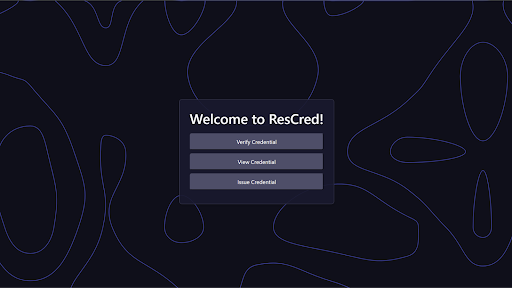
\includegraphics[width=0.95\textwidth]{img/dashboard.png}
    \end{center}
    \caption{ResCred Dashboard}\label{fig:dashboard}
\end{figure}

\begin{figure}
    \begin{center}
        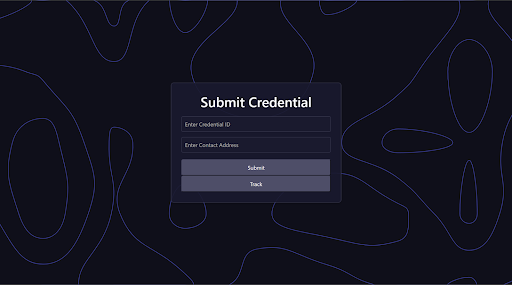
\includegraphics[width=0.95\textwidth]{img/verification_req.png}
    \end{center}
    \caption{Submit Verification Request page}\label{fig:verification_req}
\end{figure}

\begin{figure}
    \begin{center}
        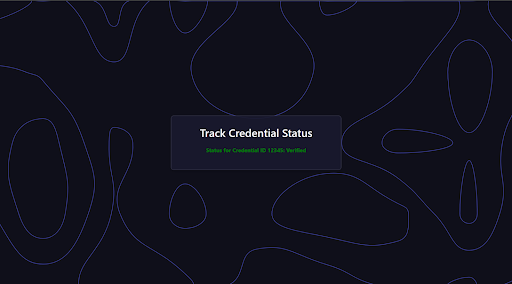
\includegraphics[width=0.95\textwidth]{img/status_verify.png}
    \end{center}
    \caption{Status of Verification Request}\label{fig:verification_status}
\end{figure}



\section{Contributions}

\begin{enumerate}
    \item Vikram - Designing the Issuing Body UI on managing credentials and registering a smart contract
    \item Fredrico - Designing and implementing the credential holder dashboard, resolving the logic for approving/rejecting credentials
    \item Avni - Implemented the frontend UI for Verifier to submit verification requests to ResilientDB and view status of a verification request. 
    \item Ethan - Frontend and GraphQL Interoperability
    \item Zhenkai - Architecture Design, Infrastructure Setup, Smart Contract Development
\end{enumerate}

All members contributed to the project and have fulfilled their share of responsibilities as
previously stated in our planning and midterm reports.


% \bibliographystyle{plain}
% \bibliography{ref}

\end{document}
